\documentclass[a4paper, 14pt,russian]{extarticle}

\usepackage[russian]{babel}
\usepackage[T2A]{fontenc}
\usepackage[utf8]{inputenc}
%Соответствующий математический шрифт для Times new roman
\usepackage{newtxmath}
\usepackage{fontspec} 
%Times new roman
\defaultfontfeatures{Ligatures={TeX},Renderer=Basic} 
\setmainfont[Ligatures={TeX,Historic}]{Times New Roman}

%Геометрия
\usepackage{geometry}
\geometry{top=20mm}
\geometry{bottom=15mm}
\geometry{left=20mm}
\geometry{right=15mm}
\usepackage{setspace}
%Нормальные дроби через запятую
\usepackage{ncccomma}

\newcommand{\changefont}{%
	\fontsize{12}{11}\selectfont
}

%Заголовки
\usepackage{fancyhdr}
\pagestyle{fancy}
\fancyhf{}
%\renewcommand{\sectionmark}[1]{\markright{#1}}
\fancyhead[R]{\changefont \slshape \leftmark}
\fancyhead[L]{\changefont \slshape \rightmark}
%\newcommand{\ssubsection}[1]{\subsection*{#1}
%	\addcontentsline{toc}{subsection}{#1}
%	\markright{#1}{}}
\cfoot{\thepage}

%\полуторный интервал
\setstretch{1.15}
\setlength{\parindent}{1.25cm}

\usepackage{amsmath, amsfonts, mathtools}
\usepackage{physics}
\usepackage{indentfirst}
\usepackage{xcolor}
\usepackage{alltt}
\usepackage{graphicx}
\usepackage{wrapfig}
%Настройка ссылок
\usepackage{hyperref}
%\usepackage{upgreek}
%\renewcommand{\beta}{\upbeta}
\hypersetup{
	colorlinks,
	citecolor=black,
	filecolor=black,
	linkcolor=black,
	urlcolor=black
}
\usepackage{caption}
\DeclareCaptionLabelSeparator{dot}{. }
\captionsetup{justification=centering,labelsep=dot}
\usepackage{titlesec}

%Формат заголовков
\titleformat{\section}{\bfseries\filcenter\Large}{\thesection}{1em}{}
\titleformat{\subsection}{\bfseries\filcenter\large}{\thesubsection}{1em}{}
\titleformat{\subsubsection}{\bfseries\filcenter\normalsize}{\thesubsubsection}{1em}{}

\usepackage{chngcntr}

%Включить в нумерацию картинок раздел
\counterwithin{figure}{section}

%Листинги кода и их стили
\usepackage{listings}
\lstdefinestyle{c++} {
	language=C++,
	breaklines=true,
	frame=single,
	numbers=left,
	basicstyle=\footnotesize\ttfamily,
	keywordstyle=\bfseries\color{green!40!black},
	commentstyle=\itshape\color{purple!40!black},
	identifierstyle=\color{blue},
	backgroundcolor=\color{gray!10!white},
}

\lstdefinestyle{python}{
	language=Python,
	breaklines=true,
	frame=single,
	numbers=left,
	basicstyle=\footnotesize\ttfamily,
	keywordstyle=\bfseries\color{green!40!black},
	frame=lines
	basicstyle=\footnotesize
}

\lstdefinestyle{cmd}{
	breaklines=true,
	frame=single,
	basicstyle=\footnotesize\ttfamily,
	frame=lines
	basicstyle=\footnotesize
}

\begin{document}
	
	\begin{titlepage}
	\newpage
	\begin{center}
		
\includegraphics[width=\textwidth]{png/tit.png}
		Институт информационных и вычислительных технологий \\
			Кафедра управления и интеллектуальных технологий
		\vspace{1.25cm}
	\end{center}
	
	\vspace{1.2em}
	
	\begin{center}
		%\textsc{\textbf{}}
		\begin{spacing}{1}
			{\Large Расчётное задание \linebreak
			По дисциплине <<Теория автоматического управления>> \\}
			\large{\bf<<Анализ нелинейных систем автоматического управления>>}
		\end{spacing}
	\end{center}
	
	\vspace{5em}
	

	\vspace{6em}
	
		\noindent Выполнил студент: Михайловский М.\,Ю. \\
		Группа: А-03-21 \\
		Вариант: 39\\
		Проверила: Сидорова Е.\,Ю.
	
	
	\vspace{\fill}
	
	\begin{center}
		Москва 2024
	\end{center}
	
\end{titlepage}
	\setcounter{page}{2}
	\pagenumbering{arabic}
	\tableofcontents
	\newpage
	
	\section{Постановка задачи}
	\subsection{Исходные данные}
	
	Дана нелинейная система со структурной схемой представленной на рис.~\ref{scheme}. Нелинейный элемент (НЭ) имеет вид двухпозиционного реле с гистерезисом с параметрами $c = 9,\,B=8$ (рис.~\ref{NE}). Передаточные функции имеют следующий вид:
	\begin{align*}
		&W_1(p) = 0,1; \\
		&W_2(p) = \frac{4}{p^2 + 3p + 9}; \\ 
		&W_3(p) = 3p.
	\end{align*}
	
	\begin{figure}[h]
		\centering\includegraphics[width=.8\textwidth]{png/схема.png}
		\caption{Структурная схема нелинейной системы}
		\label{scheme}
	\end{figure}
	\begin{figure}[h]
		\centering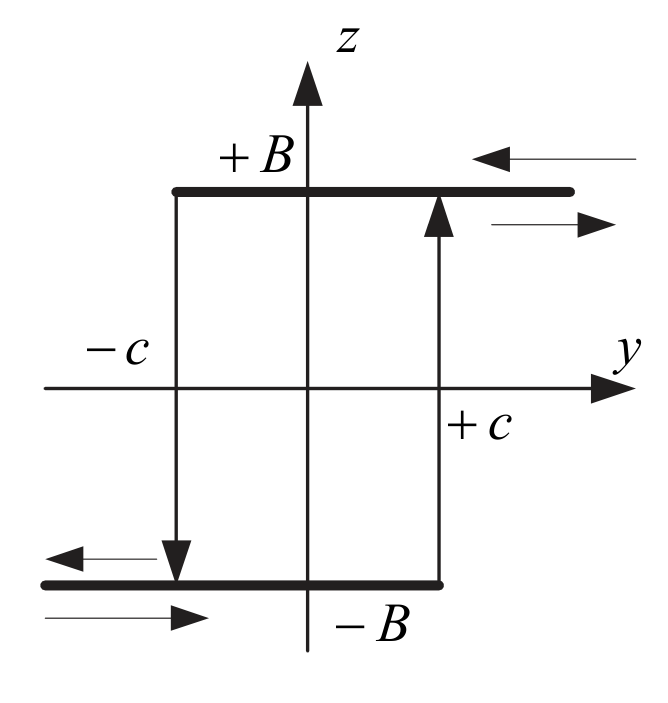
\includegraphics[width=.4\textwidth]{png/НЭ.png}
		\caption{Характеристика НЭ вида двухпозиционное реле с гистерезисом}
		\label{NE}
	\end{figure}
	
	\subsection{План исследования}
	
	\begin{enumerate}
		\item Исследовать структуру фазового портрета нелинейной системы. Для этого определить типы фазовых траекторий в различных областях фазовой плоскости. Найти описание границ данных областей, определить координаты равновесных состояний (особых точек) системы. Построить качественно ожидаемый фазовый портрет системы;
		\item С помощью стандартного ППП построить фазовый портрет системы и сравнить его с ожидаемым, полученным в п. 1. Дать заключение о характере возможных процессов в системе и их устойчивости. Определить устойчивость особых точек, наличие автоколебаний. Для трех фазовых траекторий с начальными условиями $(x_{0_1} \neq 0,\;x'_{0_1}=0)$,  $(x_{0_2} = 0,\;x'_{0_2} 
		\neq 0)$ и $(x_{0_3}\neq 0,\;x'_{0_3}\neq 0)$ привести графики изменения процесса $x(t)$ во времени;
		\item Исследовать влияние ширины петли гистерезиса нелинейного элемента на возникновение автоколебаний в системе. Определить значения параметров $c$ и $h$ НЭ 4, при которых имеют место автоколебания (другие параметры системы остаются неизменными, согласно варианту задания; см. примечание ниже). Для этого найти минимальное значение $\lambda_{\min}$ относительной величины ширины петли гистерезиса $\lambda = \dfrac{h-c}{h}\;(h>c)$, при которой возникают автоколебания. Определить амплитуду и
		период автоколебаний при $\lambda = \lambda_{\min}$;
		\item Определить амплитуду и период автоколебаний при увеличении коэффициента
		$K_1$ в 5 раз и значения $\lambda$ в 2 раза относительно $\lambda$;
		\item Провести исследование автоколебаний в системе приближенным амплитудно-частотным методом (методом Гольдфарба). Для этого привести модель системы исходной структурной схемы (рис. \ref{scheme}) к виду модели Гаммерштейна. Построить амплитудно-фазовую характеристику линейной части и инверсную характеристику $[-z(A)]$ эквивалентного
		комплексного коэффициента усиления нелинейного элемента и дать заключение о возможности возникновения автоколебаний в системе данной структуры и их устойчивости. В случае наличия автоколебаний	определить их параметры;
		
		Исследование провести для трёх случаев:
		\begin{itemize}
			\item системы с исходно заданными номером задания параметрами;
			\item системы с параметрами п. 3 при $\lambda = \lambda_{\min}$;
			\item системы с параметрами п. 4.
		\end{itemize}
		\item Сравнить количественно результаты исследования автоколебаний методом фазовой плоскости в п. 2, 3, 4 и методом Гольдфарба в п. 5.
	\end{enumerate}
	
	\section[Метод фазовой плоскости]{Исследование методом фазовой плоскости}
	\subsection{Получение фазового портрета системы}
	
	Составим уравнения системы в изображениях Лапласа:
	\begin{equation*}
		\begin{cases}
			X(p) = W_1(p)W_2(p)Z(p) = \dfrac{0,4}{p^2+3p+9}Z(p) \\
			Y(p) = W_3(p)X(p) = 3p\cdot X(p) \\
			Z(p) = \varphi(Y(p)-X(p)) = \varphi((3p-1)X(p))
		\end{cases}	
	\end{equation*}
	
	Переходя к оригиналам, получаем:
	\begin{equation}
		\begin{cases}
			x''(t) + 3x'(t) + 9x(t) = 0,4z(t) \\
			y(t) = 3x'(t) \\
			z(t) = \varphi(3x'(t) - x(t))
		\end{cases} \Rightarrow x''+3x'+9x = 0,4\varphi(3x'-x)
		\label{sys_equation}
	\end{equation}

	Аналитически выражение для НЭ задаются следующим образом:
	\begin{equation*}
		z(t) = \varphi(y) = \begin{cases}
			8, &y\geq 9 \\
			8, &-9\geq y \geq 9,\;(z^{-} = 8) \\
			-8, &-9 \geq y \geq 9,\;(z^{-}=-8) \\ 
			-8, &y \leq -9
		\end{cases},\;\text{где } z^{-} = \lim_{\xi\to 0}z(t-\xi)
	\end{equation*}
	
	Перейдём к представлению системы в переменных состояния сделав замену $x'(t) = v(t)$:
	\begin{equation}
		\begin{cases}
			\dv{x}{t} = v \\
			\dv{v}{t} = \begin{cases}
				3,2-3v-9x, &3v-x\geq 9 \\
				3,2-3v-9x, &-9\geq 3v-x \geq 9,\;(z^{-} = 8) \\
				-3,2-3v-9x, &-9 \geq 3v-x \geq 9,\;(z^{-} = -8) \\ 
				-3,2-3v-9x, &3v-x \leq -9
			\end{cases}
		\end{cases}
		\label{sys_equations}
	\end{equation}
	
	Отсюда полупрямые переключения будут следующие:
	\begin{equation}
		\left[\begin{aligned}
			&3v-x = 9,\,v\geq 0 \\
			&3v-x = -9,\,v\leq 0 
		\end{aligned}\right.
		\label{perekl}
	\end{equation}
	
	Исследуем характер фазовых траекторий для произвольного значения $z(t) = C$. Рассмотрим уравнение (\ref{sys_equation}):
	\begin{equation}
		x''+3x'+9x = C \Rightarrow x'' + 3x' + 9\left(x-\frac{C}{9}\right) = 0
		\label{obsh_ur}
	\end{equation}
	 
	Уравнение (\ref{obsh_ur}) представляет собой сдвинутые по $x$ на $\frac{C}{9}$ вправо фазовые траектории линейной системы, заданной следующим характеристическим уравнением (ХУ):
	\begin{equation*}
		p^2 + 3p + 9 = 0 \Rightarrow p_{1,\,2} = \frac{-3\pm\sqrt{3^2 - 4\cdot9}}{2} = -\frac{3}{2} \pm j\frac{3\sqrt{3}}{2}
	\end{equation*}
	
	Такие корни ХУ соответствуют особой точке типа устойчивый фокус. Переходной процесс будет иметь следующий вид:
	\begin{equation*}
		x(t) = \frac{C}{9} + Ae^{-\frac{3}{2}t}\sin(\frac{3\sqrt{3}}{2}t + \theta)
	\end{equation*}
	Здесь значения $A,\,\theta$ зависят от начальных условий.
	
	НЭ в рассматриваемой системе может принимать 2 значения, поэтому будет два типа фазовых траекторий. 
	
	Пусть $z(t) = 8$ задаёт траектории I типа. Из (\ref{obsh_ur}) видно, что для этого случая $C=8$. Тогда $z(t) = -8$ задаёт траектории II типа и $C = -8$.
	
	Нарисуем качественно вид траекторий. Учитывая сдвиг по оси $x$ на $\dfrac{C}{9}$, особыми точками будут  $\left(\dfrac{8}{9},\,0\right)$ и $\left(-\dfrac{8}{9},\,0\right)$ для I и II типа фазовых траекторий соответственно. Полученные траектории показаны на рис. \ref{tracks}.
	
	
	\noindent\begin{minipage}{.5\textwidth}
		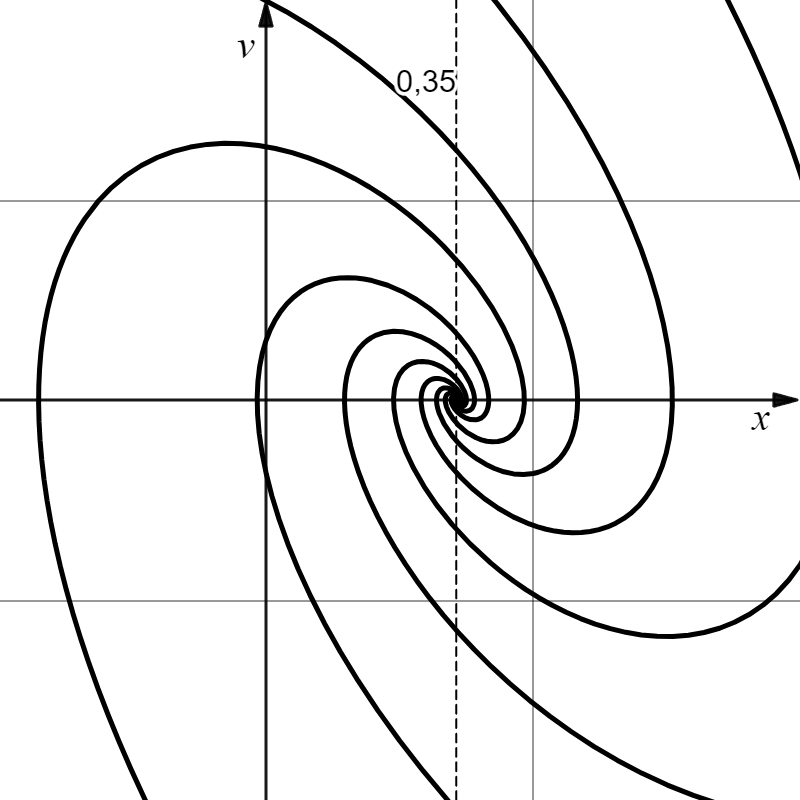
\includegraphics[width=\textwidth]{png/траектории1.png}
		\centering I тип
	\end{minipage}
	\begin{minipage}{.5\textwidth}
		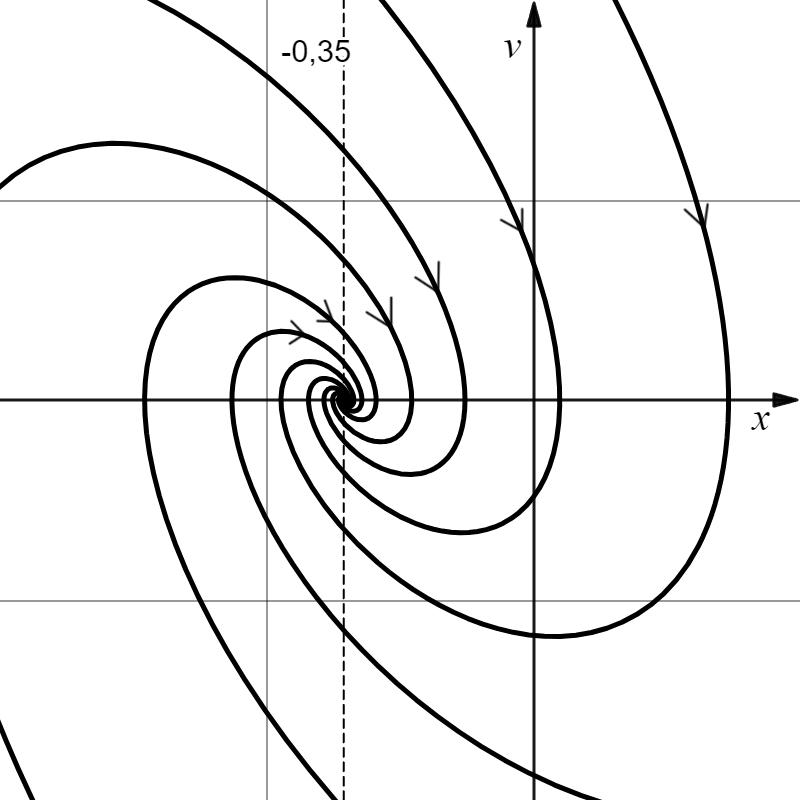
\includegraphics[width=\textwidth]{png/траектории2.png}
		\centering II тип
	\end{minipage}
	\captionof{figure}{Фазовые траектории I и II типов}
	\label{tracks}

\end{document}
